\documentclass[twoside,10pt]{article}
\usepackage{xparse}
\usepackage[margin=0.9in]{geometry}
\usepackage{tcolorbox}
\setlength\parindent{0pt}
\definecolor{bubblegum}{rgb}{0.99, 0.76, 0.8}
\usepackage[normalem]{ulem}
\usepackage{xcolor,colortbl}
\usepackage{framed}
\usepackage{caption}
\usepackage{subcaption}
\captionsetup{font={small}}
\usepackage{amsmath}
\usepackage{amssymb}
\usepackage{graphicx}
\usepackage{listings}
\usepackage{lipsum}
\usepackage{courier}
\usepackage{xcolor}
\usepackage{graphicx}

\definecolor{backcolour}{rgb}{0.95,0.95,0.92}

\lstdefinestyle{mystyle}{
    backgroundcolor=\color{backcolour},
    basicstyle=\ttfamily\normalsize,
    breakatwhitespace=false,         
    breaklines=true,                 
    captionpos=b
}
\lstset{style=mystyle}


\begin{document}

\begin{center}
    {\Large \bf CS 682 – Artificial Intelligence}

    \vspace{.5cm}

    {\Large \bf Project 3 – Reinforcement Learning}

    \vspace{0.5cm}
    {\large \bf Monikrishna Roy}
    \vspace{0.5cm}

    {\large \today}

\end{center}

\subsection*{Objectives}\label{objectives}

To implement a reinforcement learning algorithm that can learn a policy
for a given task based on task-based rewards. To take a continuous
environment and discretize it so that it is suitable for a reinforcement
learning task.


\subsection*{Task Description}\label{task-description}

\begin{center}
    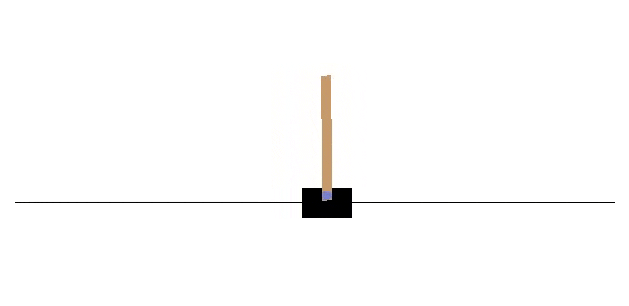
\includegraphics[width=8cm]{figs/cartPole.png}
\end{center}

This is the CartPole task. The idea here is to balance this pole using a
one-dimensional action (it can only move left and right). The agent's
state has 4 components:

\begin{itemize}

    \item
          x: the location of the robot (0 is the center, -2.4 is the leftmost
          part of the board, 2.4 is the rightmost part of the board)
    \item
          xdot: the velocity of the robot (technically, this can go from -inf to
          inf)
    \item
          theta: the angle that the pole is at (0 is straight up, -12 degrees or
          fewer means that the pole falls to the left, 12 degrees or more means
          that the pole falls to the right)
    \item
          thetadot: the change in angle per second.
\end{itemize}

The robot can choose between two actions:

\begin{itemize}
    \item
          0: move left
    \item
          1: move right
\end{itemize}

Success is balancing for 200 ticks, failure is if the stick falls more
than 12 degrees from the median, or if the robot moves more than 2.4
meters from the center.


\subsubsection*{Example Code}\label{example-code}

In the Canvas,

\begin{quote}
    Files-\textgreater{}Projects-\textgreater{}Project
    2-\textgreater{}cart.py
\end{quote}

\begin{quote}
    For training, call: python3 cart.py --train
\end{quote}

\begin{quote}
    For testing, call: python3 cart.py --test --model \textless{}model
    file\textgreater{}
\end{quote}


\subsubsection*{OpenAI Gym}\label{openai-gym}

You do not have to implement the problem domain yourself, there is a
resource called openAI gym which has a set of common training examples.
Gym can be installed on unix based system with the following command:

\begin{quote}
    sudo -H pip3 install gym
\end{quote}

After running the provided command, you may also be asked to install
some additional packages for the video encoding. You'll see an error
message with instructions to follow.

\subsubsection*{State Discretization}\label{state-discretization}

We will discretize the space in order to simplify the reinforcement
learning algorithm. For each state we determine the realistic minimum
and maximum values and store it in arrays MIN\_VALS and MAX\_VALS
respectively (line 14 and 15). These arrays are then used to discretize
each element of the state into respective NUM\_BINS (line 16). For
example, state(0) i.e., position (x) with minimum and maximum value of
\(-2.5\) and \(+2.5\), respectively, is discretized into 9 bins in the
example code (cart.py) which implies that for x\textless{}-2.5 will be
one bucket, \(-2.5<x<-1.875\) will be another and so on.

These state components are encoded into a single integer state
\((0 ... 9999)\). This is done for you in the function discretize\_state
in the provided code.


\subsection*{Task (part 1)}\label{task-part-1}

You need to implement the q-learning part of this task (right now the
example code will not do any learning). You need to implement the
following equation from the lecture slides:

\begin{quote}
    Q-values can be learned directly from reward feedback

    \[Q(a,s) <- Q(a,s) + \alpha(R(s) + \gamma * max_{a'}(Q(a',s') - Q(a,s)))\]
\end{quote}

Here, \(s\) is the current state, \(s'\) (sprime) is the next state, and
a is the current action. The above equation needs to be implemented on
line 142. Reward is stored in the variable reward, and the learning rate
\((\alpha)\) is in the variable alpha, which is set on line 101. The
predicted value of the next state, \(max_{a'}Q(a',s')\), is already
computed and stored in the variable predicted\_value.

You'll need to implement the equation on line 142 and tune the values of
the parameters alpha and gamma (lines 101 and 101, respectively). You
should only have to write one line of code and adjust some values for
this part. It is suggested that you step the alpha (learning rate)
values up and down by factors of .1 in both directions and the gamma
values by .1 in both directions to see the effect it has on the
learning. Usually learning rate is kept low such that the policy does
not take huge step toward convergence and miss the local minima,
eventually diverging from it. Gamma, on the other hand, represents the
discount factor which essentially means how much the policy prefers
current reward over future rewards.

The program will train over 50001 episodes and play a video of each
1000th training.

This is easy on the code side and will allow you to experiment with the
various factors of reinforcement learning.

\subsection*{Task (part 2)}\label{task-part-2}

\begin{center}
    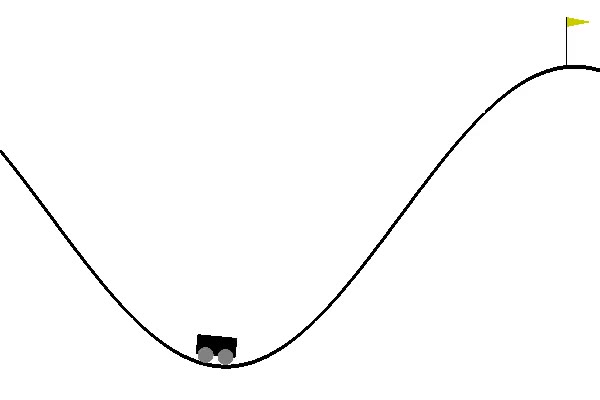
\includegraphics[width=8cm]{figs/mountainCar.jpg}
\end{center}

Now that you've implemented q-learning for one task, you will move to
the mountain car task. Instead of 2 actions (left, right), this task has
three (left, null, right). The task also has different state variables
(only 2 for mountain car)

\begin{itemize}

    \item
          x: the location of the robot (\(-1.2\) is the left, \(-.45\) is
          approximately the valley, \(0.6\) is the rightmost part of the board,
          \(0.5\) is the location of the flag)
    \item
          xdot: the velocity of the robot (this can go from \(-0.07\) to
          \(0.07\))
\end{itemize}

This will require you to change the following:

\begin{itemize}
    \item
          Q-function, Gamma, Alpha:

          \begin{itemize}
              \item
                    First, similar to Part 1, copy the working Q-function and parameters
                    from Part 1 to car.py
          \end{itemize}
    \item
          Minimum values, maximum values and number of bins:

          \begin{itemize}

              \item
                    MIN\_VALS = {[} {]}
              \item
                    MAX\_VALS = {[} {]}
              \item
                    NUM\_BINS = {[} {]}
          \end{itemize}
    \item
          Total number of possible states:

          Depending on the NUM\_BINS, you need to set the number of possible
          states. For example, in the cartpole problem in Part I, there was
          \(10\) bins for each variable, leading to
          \(10 * 10 * 10 * 10 - 1 = 9999\) states. Now you have \(2\) variables.
          Assuming that you have Y bins for each variable, you will end up with
          \(Y*Y-1\) states. Replace \(9999\) in line 87 with the appropriate
          number whenever you change the values in NUM\_BINS.
\end{itemize}


\subsection*{Implementation}\label{implementation}

\subsubsection*{Part 1}\label{part-1}

After a few trying of tunning parameters, we got a good result for the
cartpole problem for the following parameters:

\begin{verbatim}
- alpha = 0.1
- gamma = 0.9
\end{verbatim}

The code for Part 1 is provided in the file cart.py. You can run the
code by calling:

\begin{verbatim}
> python3 cart.py --train
\end{verbatim}

The model file is also provided in the project and saved as cart.npy.
You can use it to test the code by calling:

\begin{verbatim}
> python3 cart.py --test --model cart.npy
\end{verbatim}


\subsubsection*{Part 2}\label{part-2}

For the mountain car problem, we will use the following parameters:

\begin{verbatim}
- alpha = 0.5
- gamma = 0.9
\end{verbatim}

Minimum values, maximum values and number of bins:

\begin{verbatim}
- MIN_VALS = [-1.2, -0.07]
- MAX_VALS = [0.6, 0.07]
- NUM_BINS = [100, 100]
\end{verbatim}

The code for Part 2 is provided in the file car.py. You can run the code
by calling:

\begin{verbatim}
> python3 car.py --train
\end{verbatim}

The model file is also provided in the project and saved as car.npy. You
can use it to test the code by calling:

\begin{verbatim}
> python3 car.py --test --model car.npy
\end{verbatim}

\end{document}
